\documentclass{lab}
\graphicspath{{pics/}}

\title {Лабораторная работа 3.5.1}
\author {Сидорчук Максим Б01-304}
\date{\today}

\begin  {document}
\maketitle
\section*{Теория}
\subsection*{Плазма}

Из-за теплового движения в плазме электроны могут смещаться относительно ионов и образовывать неоднородности. В этих неоднородностях возникает электрическое поле, которое стремится восстановить баланс, из-за чего происходят колебания с частотой
\[w_p = \sqrt{\frac{4\pi n_e e^2}{m_e}}\]
За характерное время колебаний электроны за счет теплового движения смещаются на
\[r_D \sim \frac{v_e}{w_p} = \sqrt{\frac{kT_e}{4\pi n_e e^2}}\]
$r_D$ - дебаевский радиус, $k$ - константа Больцмана.\\
Если поместить в плазму пробную (допустим, положительную) частицу, то электроны будут скапливаться около этой частицы, экранируя её поле. Потенциал точечного заряда будет иметь в плазме следующий вид:
\[\varphi(r) = \frac{q}{r}e^{-\frac{r}{r_D}}\]
где $r_D = \sqrt{\dfrac{kT_e}{4\pi n e^2}}$ -- \textit{радиус Дебая в случае равновесной плазмы}. Если температуры электронов и ионов сильно отличаются, то следует определять отдельно величину радиуса экранирования для электронов и для ионов. Итоговый радиус будет
\[r_D = (r_{De}^{-2} + r_{Di}^{-2})^{-1/2}\]
То есть если $T_i \ll T_e$, то $r_D \approx r_{Di}$
\subsection*{Одиночный зонд}
При внесении в плазму уединённого проводника -- \textit{зонда} -- с потенциалом, изначально равным потенциалу точки плазмы, в которую его помещают, на него поступают токи электроннов и ионов:
\begin{equation}
    \begin{array}{c}
        I_{e0} = \dfrac{n \langle v_e \rangle}{4}eS,\\
        I_{i0} = \dfrac{n \langle v_i \rangle}{4}eS,
    \end{array}
\end{equation}
где $\langle v_e \rangle$ и $\langle v_i \rangle$ -- средние скорости электронов и ионов, $S$ -- площадь зонда, $n$ -- плотность электронов и ионов. Скорости электронов много больше скорости ионов, поэтому $I_{i0} \ll I_{e0}$. Зонд будет заряжаться до некоторого равновестного напряжения $-U_f$ -- \textit{плавающего потенциала}.\\
В равновесии ионный ток мало меняется, а электронный имеет вид
$$
I_e = I_0 \exp\left( -\dfrac{eU_f}{kT_e} \right).
$$
Будем подавать потенциал $U_\text{з}$ на зонд и снимать значение зондового тока $I_\text{з}$. Максимальное значение тока $I_{e\text{н}}$ -- электронный ток насыщения, а минимальное $I_{i\text{н}}$ -- ионный ток насыщения. Значение из эмпирической формулы Бомона:
\begin{equation}
    I_{i\text{н}} = 0.4 neS \sqrt{\dfrac{2kT_e}{m_i}}.
\end{equation}

Электронный ток насыщения можно определить по тепловому движению:
\[I_{e\text{н}} = \frac{n_eS}{4}\sqrt{\frac{8kT}{\pi m_e}}\]
\subsection*{Двойной зонд}
Двойной зонд -- система из двух одинаковых зондов, расположенных на небольшом расстоянии друг от друга, между которыми создаётся разность потенциалов, меньшая $U_f$. Рассчитаем ток между ними вблизи $I=0$. При небольших разностях потенциалов ионные токи на оба зонда близки к току насыщения и компенсируют друг друга, а значит величина результирующего тока полностью связана с разностью электронных токов. Пусть потенциалы на зондах
$$
U_1 = -U_f + \Delta U_1,
$$
$$
U_2 = -U_f + \Delta U_2.
$$
Между зондами $U = U_2 - U_1 = \Delta U_2 - \Delta U_1$.
Через первый электрод
\begin{equation}
    I_1 = I_{i\text{н}} + I_{e1} = I_{i\text{н}} - \dfrac{1}{4}neS\langle v_e\rangle \exp\left(-\dfrac{eU_f}{kT_e}\right)\exp\left(\dfrac{e\Delta U_1}{kT_e}\right)=I_{i\text{н}}\left(1 - \exp\left( \dfrac{e\Delta U_1}{kT_e} \right)\right).
\end{equation}
Аналогично через второй получим
\begin{equation}
    I_2 = I_{i\text{н}}\left(1 - \exp\left( \dfrac{e\Delta U_2}{kT_e} \right)\right)
\end{equation}

Из $(7)$ и $(8)$ с учётом последовательного соединение зондов ($I_1 = -I_2 = I)$:
$$
\Delta U_1= \dfrac{kT_e}{e}\text{ln}\left(1 - \dfrac{I}{I_{i\text{н}}}\right)
$$
$$
\Delta U_2= \dfrac{kT_e}{e}\text{ln}\left(1 + \dfrac{I}{I_{i\text{н}}}\right)
$$

Тогда итоговые формулы для разности потенциалов и тока

\begin{equation}
    U = \dfrac{kT_e}{e}\text{ln}\dfrac{1 - I/I_{i\text{н}}}{1 + I/I_{i\text{н}}}, \ \
    I = I_{i\text{н}} \text{th}\dfrac{eU}{2kT_e}.
\end{equation}

\begin{wrapfigure}[5]{l}{0.4\textwidth}
    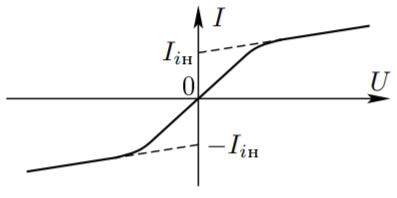
\includegraphics[scale=0.8]{4.png}
\end{wrapfigure}
Зависимость выглядит примерно так.
Из формулы можно найти формулу для $T_e$: для $U=0$ мы найдём $I_{i\text{н}}$, продифференцируем в точке $U=0$ и с учётом $\text{th}~\alpha \approx \alpha$ при малых $\alpha$ и $A\rightarrow 0$ получим:
\begin{equation}
    kT_e = \dfrac{1}{2}\dfrac{eI_{i\text{н}}}{\dfrac{dI}{dU}|_{U=0}}.
\end{equation}
\section*{Описание установки}
\begin{center}
    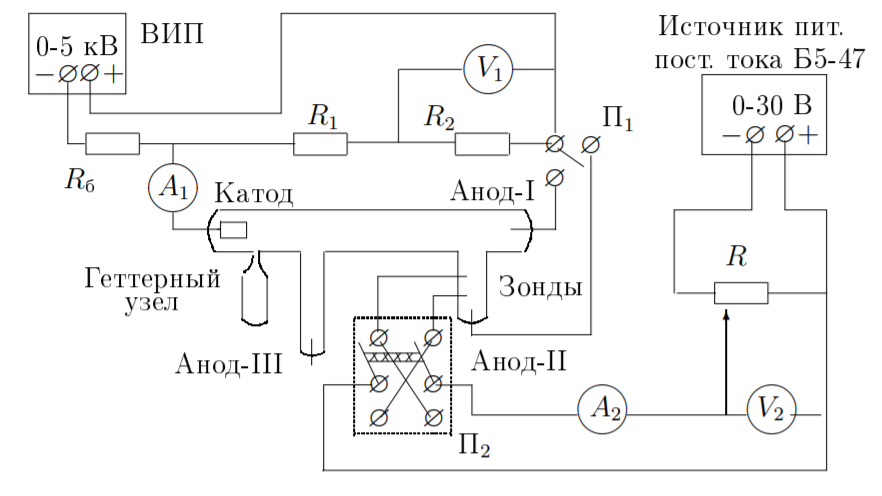
\includegraphics[scale=0.9]{1.png}
\end{center}
Стеклянная газоразрядная трубка имеет холодный (ненакаливаемый) полый катод, три анода и \textit{геттерный} узел -- стеклянный баллон, на внутреннюю повехность которого напылена газопоглощающая плёнка (\textit{геттер}). Трубка наполнена изотопом неона $^22$Ne при давлении 2 мм рт. ст. Катод и один из анодом (I и II) с помощью переключателя $\Pi_1$ подключается через балластный резистор $R_\text{б}$ ($\approx 450$ кОм) к регулируемому ВИП с выкодным напряжением до 5 кВ.\\
При подключении к ВИП анода-I между ним и катодом возникает газовый разряд. Ток разряда измеряется миллиамперметром $A_1$, а падение напряжения на разрядной трубке -- цифровым вольтметром $V_1$, подключённым к трубке черезе высокоомный (25 МОм) делитель напряжения с коэффициентом $(R_1+R_2)/R_2 = 10$.\\
При подключении к ВИП анода-II разряд возникает в пространстве между катодом и анодом-II, где находятся двойной зонд, используемый для диагностики плазмы положительного столба. Зонды изготовлены из молибденовой проволоки диаметром $d = 0.2$ мм и имеют длину $l = 5.2$ мм. Они подключены к источнику питания GPS через потенциометр $R$. Переключатель $\Pi_2$ позволяет изменять полярность напряжения на зондах. Величина напряжения на зондах изменяеься с помощью дискретного переключателя <<$V$>> выходного напряжения источника питания и потенциометра $R$, а измеряется цифровым вольтметром $V_2$. Для измерения зондового тока используется мультиметр $A_2$.

\section*{Ход работы}
\subsection{Одиночный зонд}
Измеряем напряжение зажигания в лампе: $U_{\text{заж}} \approx 215 $ В.\\
Снимаем ВАХ газового разряда:
\begin{table}[H]
    \centering
    \begin{tabular}{|c|c|}
        \hline
        $I$, мА & $U$, В \\\hline
        0.305 & 360.00 \\ \hline
        0.463 & 351.76 \\ \hline
        0.587 & 348.60 \\ \hline
        0.705 & 344.47 \\ \hline
        0.795 & 341.13 \\ \hline
        0.904 & 335.13 \\ \hline
        1.061 & 317.66 \\ \hline
        1.208 & 294.55 \\ \hline
        1.390 & 272.79 \\ \hline
        1.590 & 259.60 \\ \hline
        1.810 & 248.95 \\ \hline
        2.001 & 240.16 \\ \hline
        2.532 & 223.12 \\ \hline
        3.019 & 207.42 \\ \hline
        3.520 & 199.40 \\ \hline
        4.047 & 196.35 \\ \hline
        4.516 & 192.93 \\ \hline
        5.007 & 189.70 \\ \hline
    \end{tabular}
\end{table}

Построим АВХ и определим максимальное дифференциальное сопротивление разряда $R_{\text{диф}} = \frac{dU}{dI}$. Оно будет соответствовать участку с максимальным (по модулю) наклоном графика $U{I}$:

\begin{figure}[H]
    \centering
    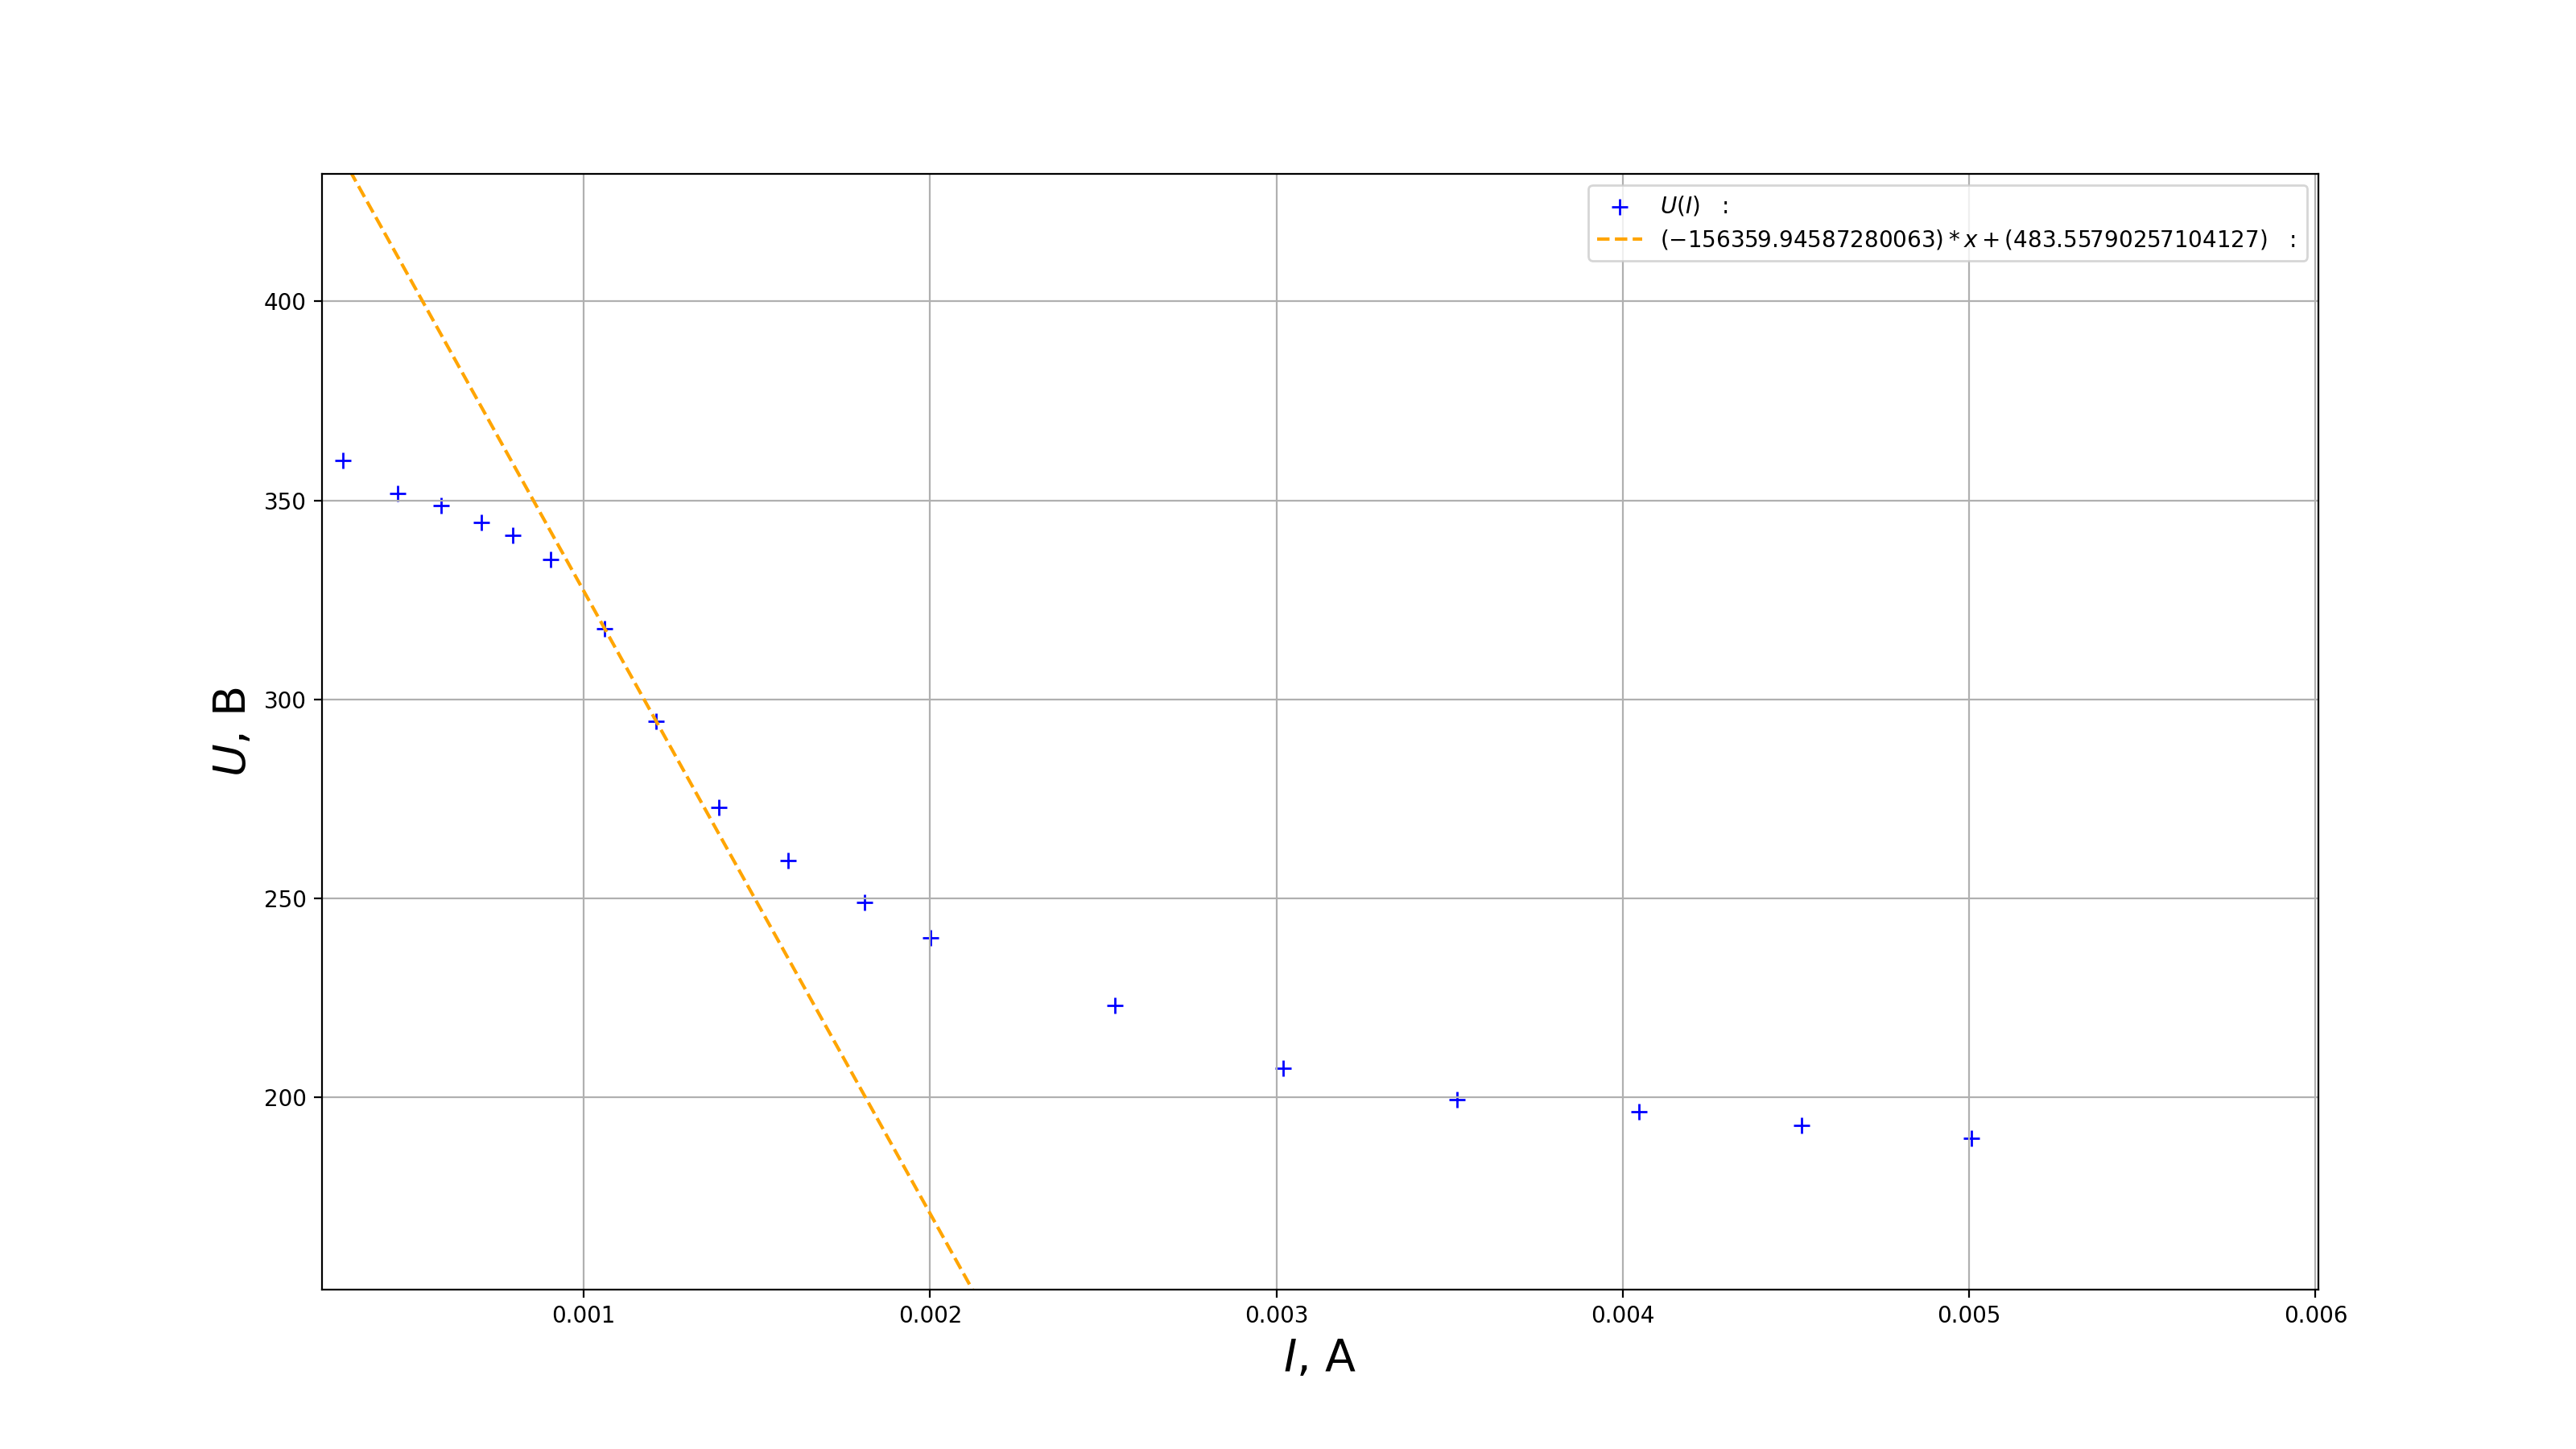
\includegraphics[width = \textwidth]{graph1.png}
    \caption{АВХ газового разряда в неоне}
\end{figure}
Получаем (с учетом делителя и порядка величин) $R_{\text{диф}} \approx 1.56 \cdot 10^5$ Ом. Наш график соответствует участку поднормального тлеющего разряда (см. приложение к лабораторной работе), а при токе $I \approx 3$ мА он начинает переходить в нормальный тлеющий разряд.

С помощью вольтметра $V_2$ и амперметра $A_2$ снимем ВАХ двойного зонда $I_2 = f(U_2)$ при фиксированном токе разряда $I_p$ в трубке в диапозоне $-25 \div 25$ В, процессе измерений меняя полярность зонда при нулевом токе. Измерения проведём для $I_p = 5,02$ мА, $I_p = 3,02$ мА  и $I_p = 1,522$ мА.

\begin{figure}[H]
    \centering
    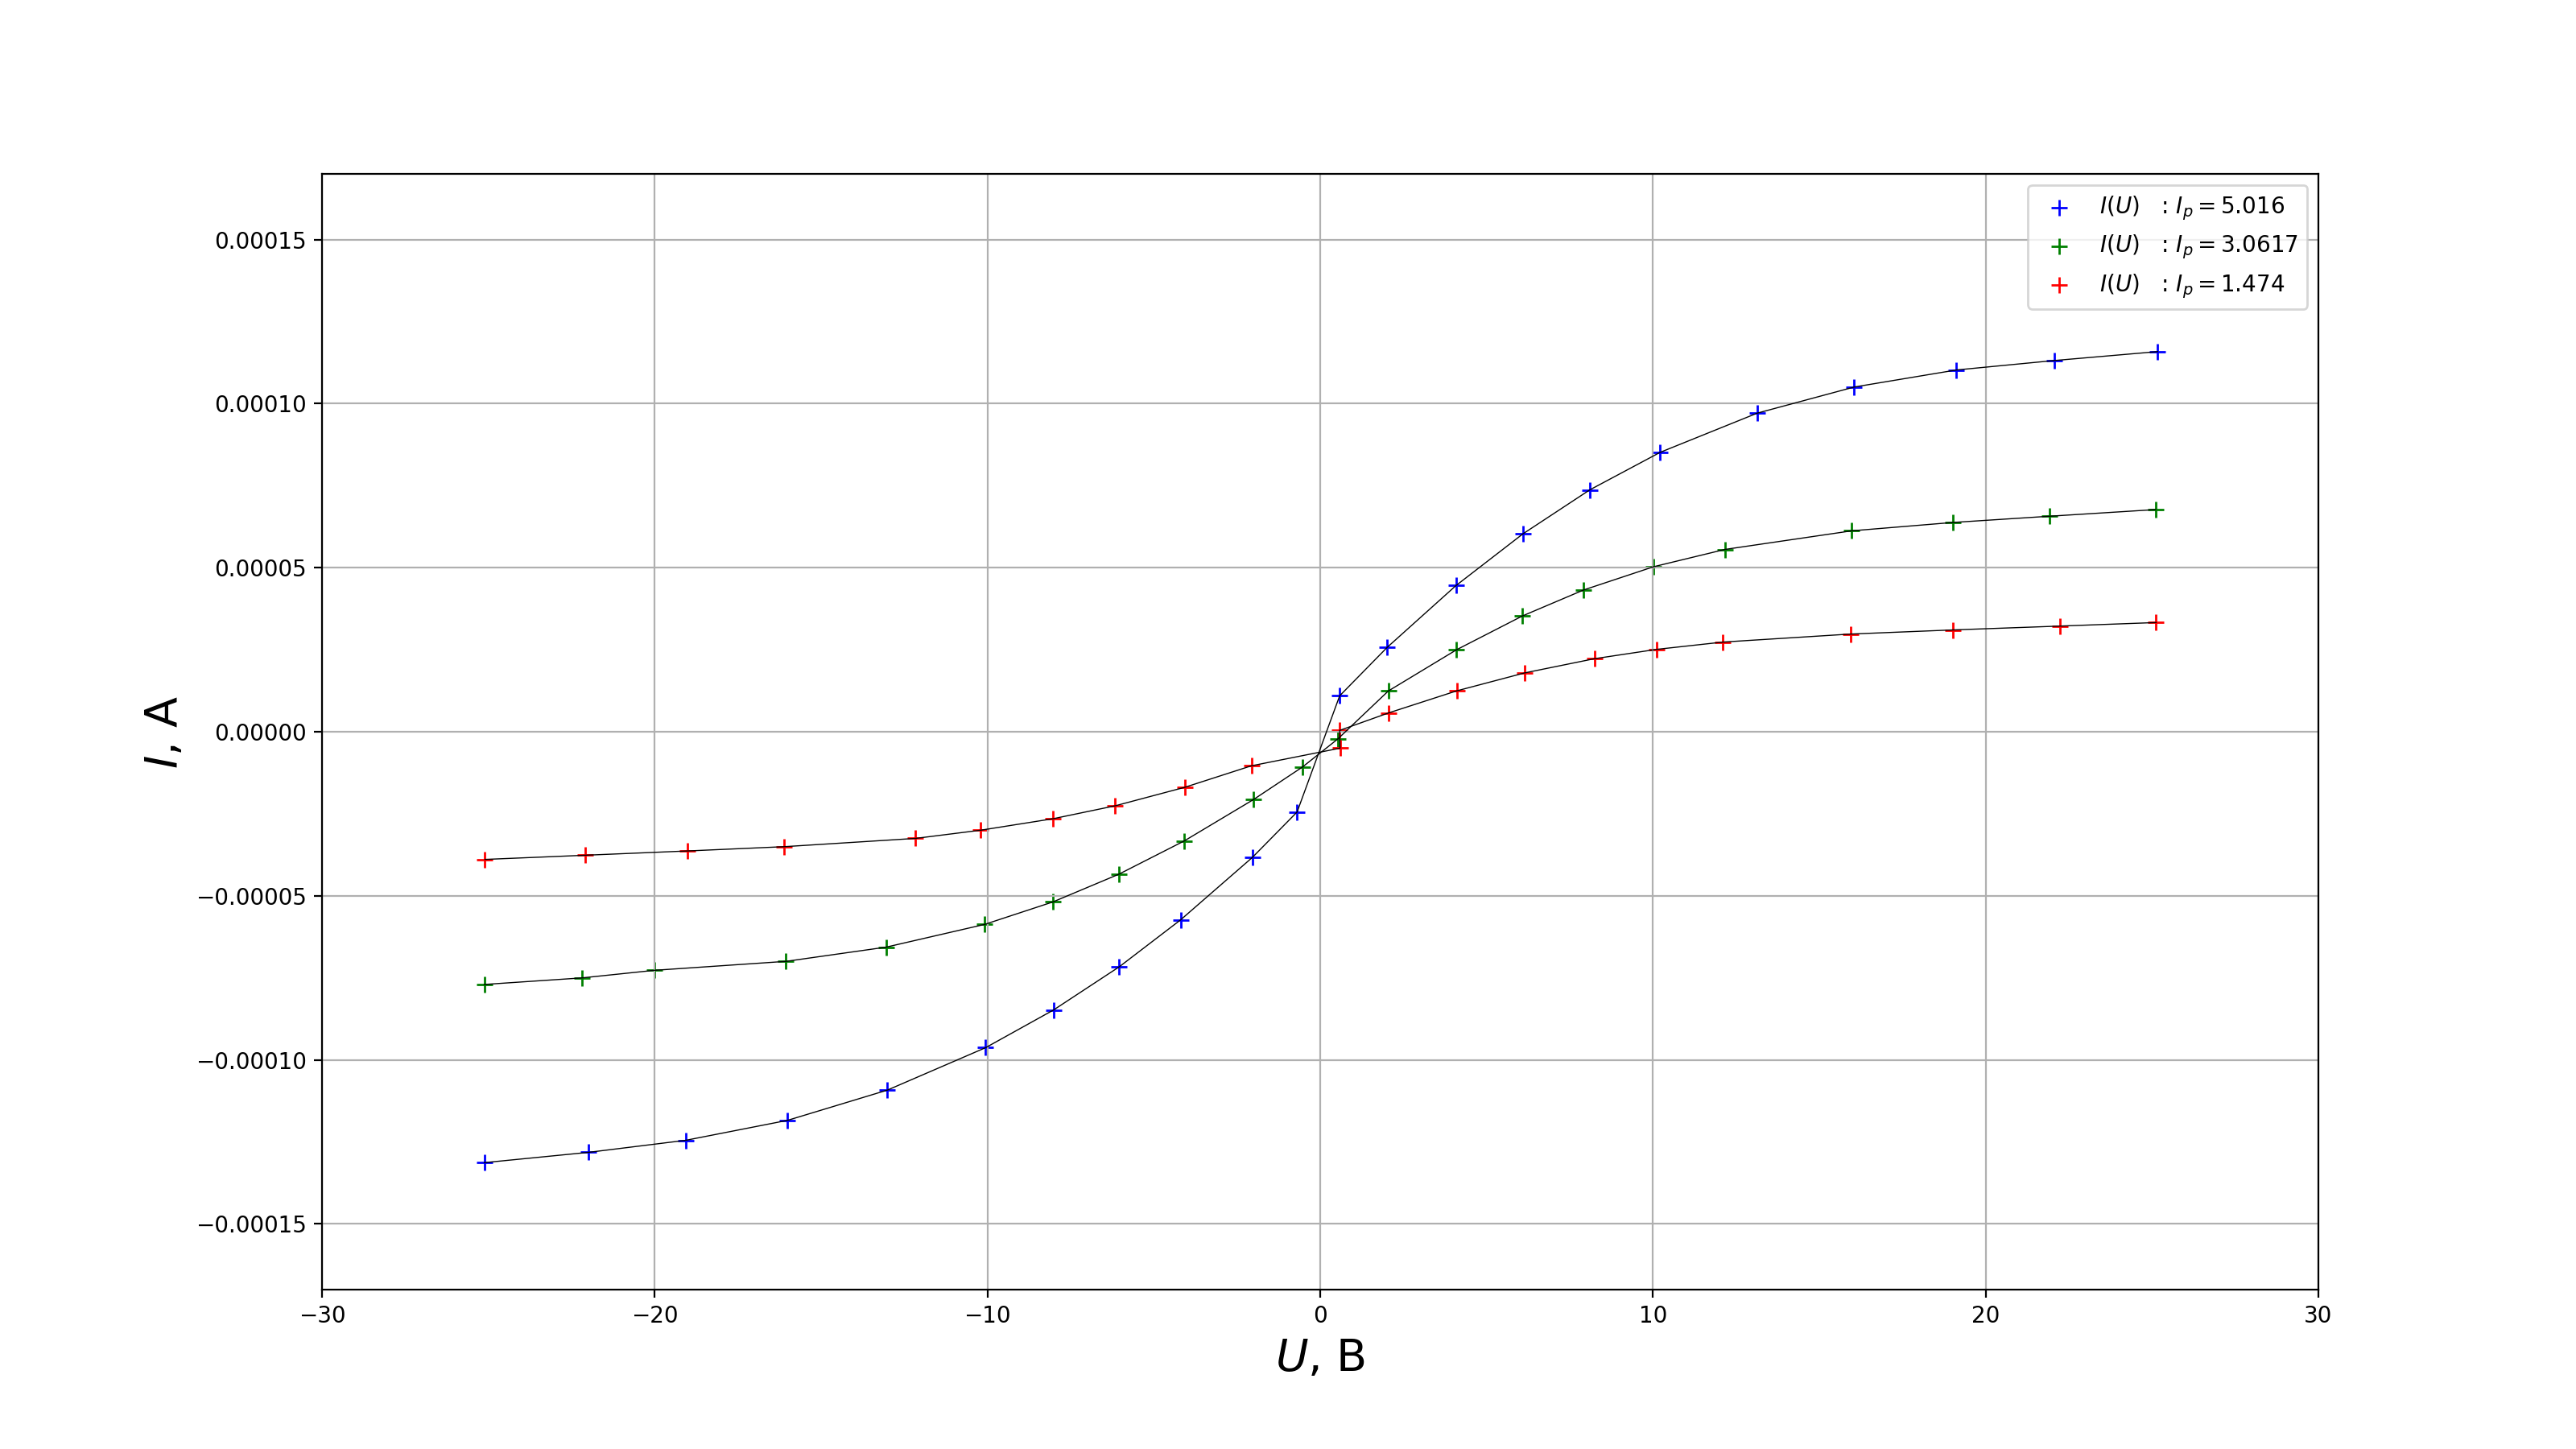
\includegraphics[width = \textwidth]{graph2.png}
\end{figure}

Видно, что чем меньше ток, тем менее крутая кривая получается. Проанализируем графики по отдельности, чтобы найти их наклон в начале и пересечение асимптот с осью ординат. Данные будем заносить в таблицу. Ионный ток насыщения определим через асимптоты, затем по наклону кривой в точке $U = 0$ найдем концентрацию электронов в плазме.

При токе $I_p = 5,02$ мА первая и последняя точка несколько выбиваются из зависимости, скорее всего, потому что $I_p$ изменялся во время проведения эксперимента и к концу измерений на этом токе бл $I_p = 5,078$ мА. Эти точки мы убрали из рассмотрения. В оставшихся измерениях ток $I_p$ менялся не очень сильно. В дальнейших измерениях будем брать значения тока насыщения ионов, измеренные по верхней ветке.

\begin{figure}[H]
    \centering
    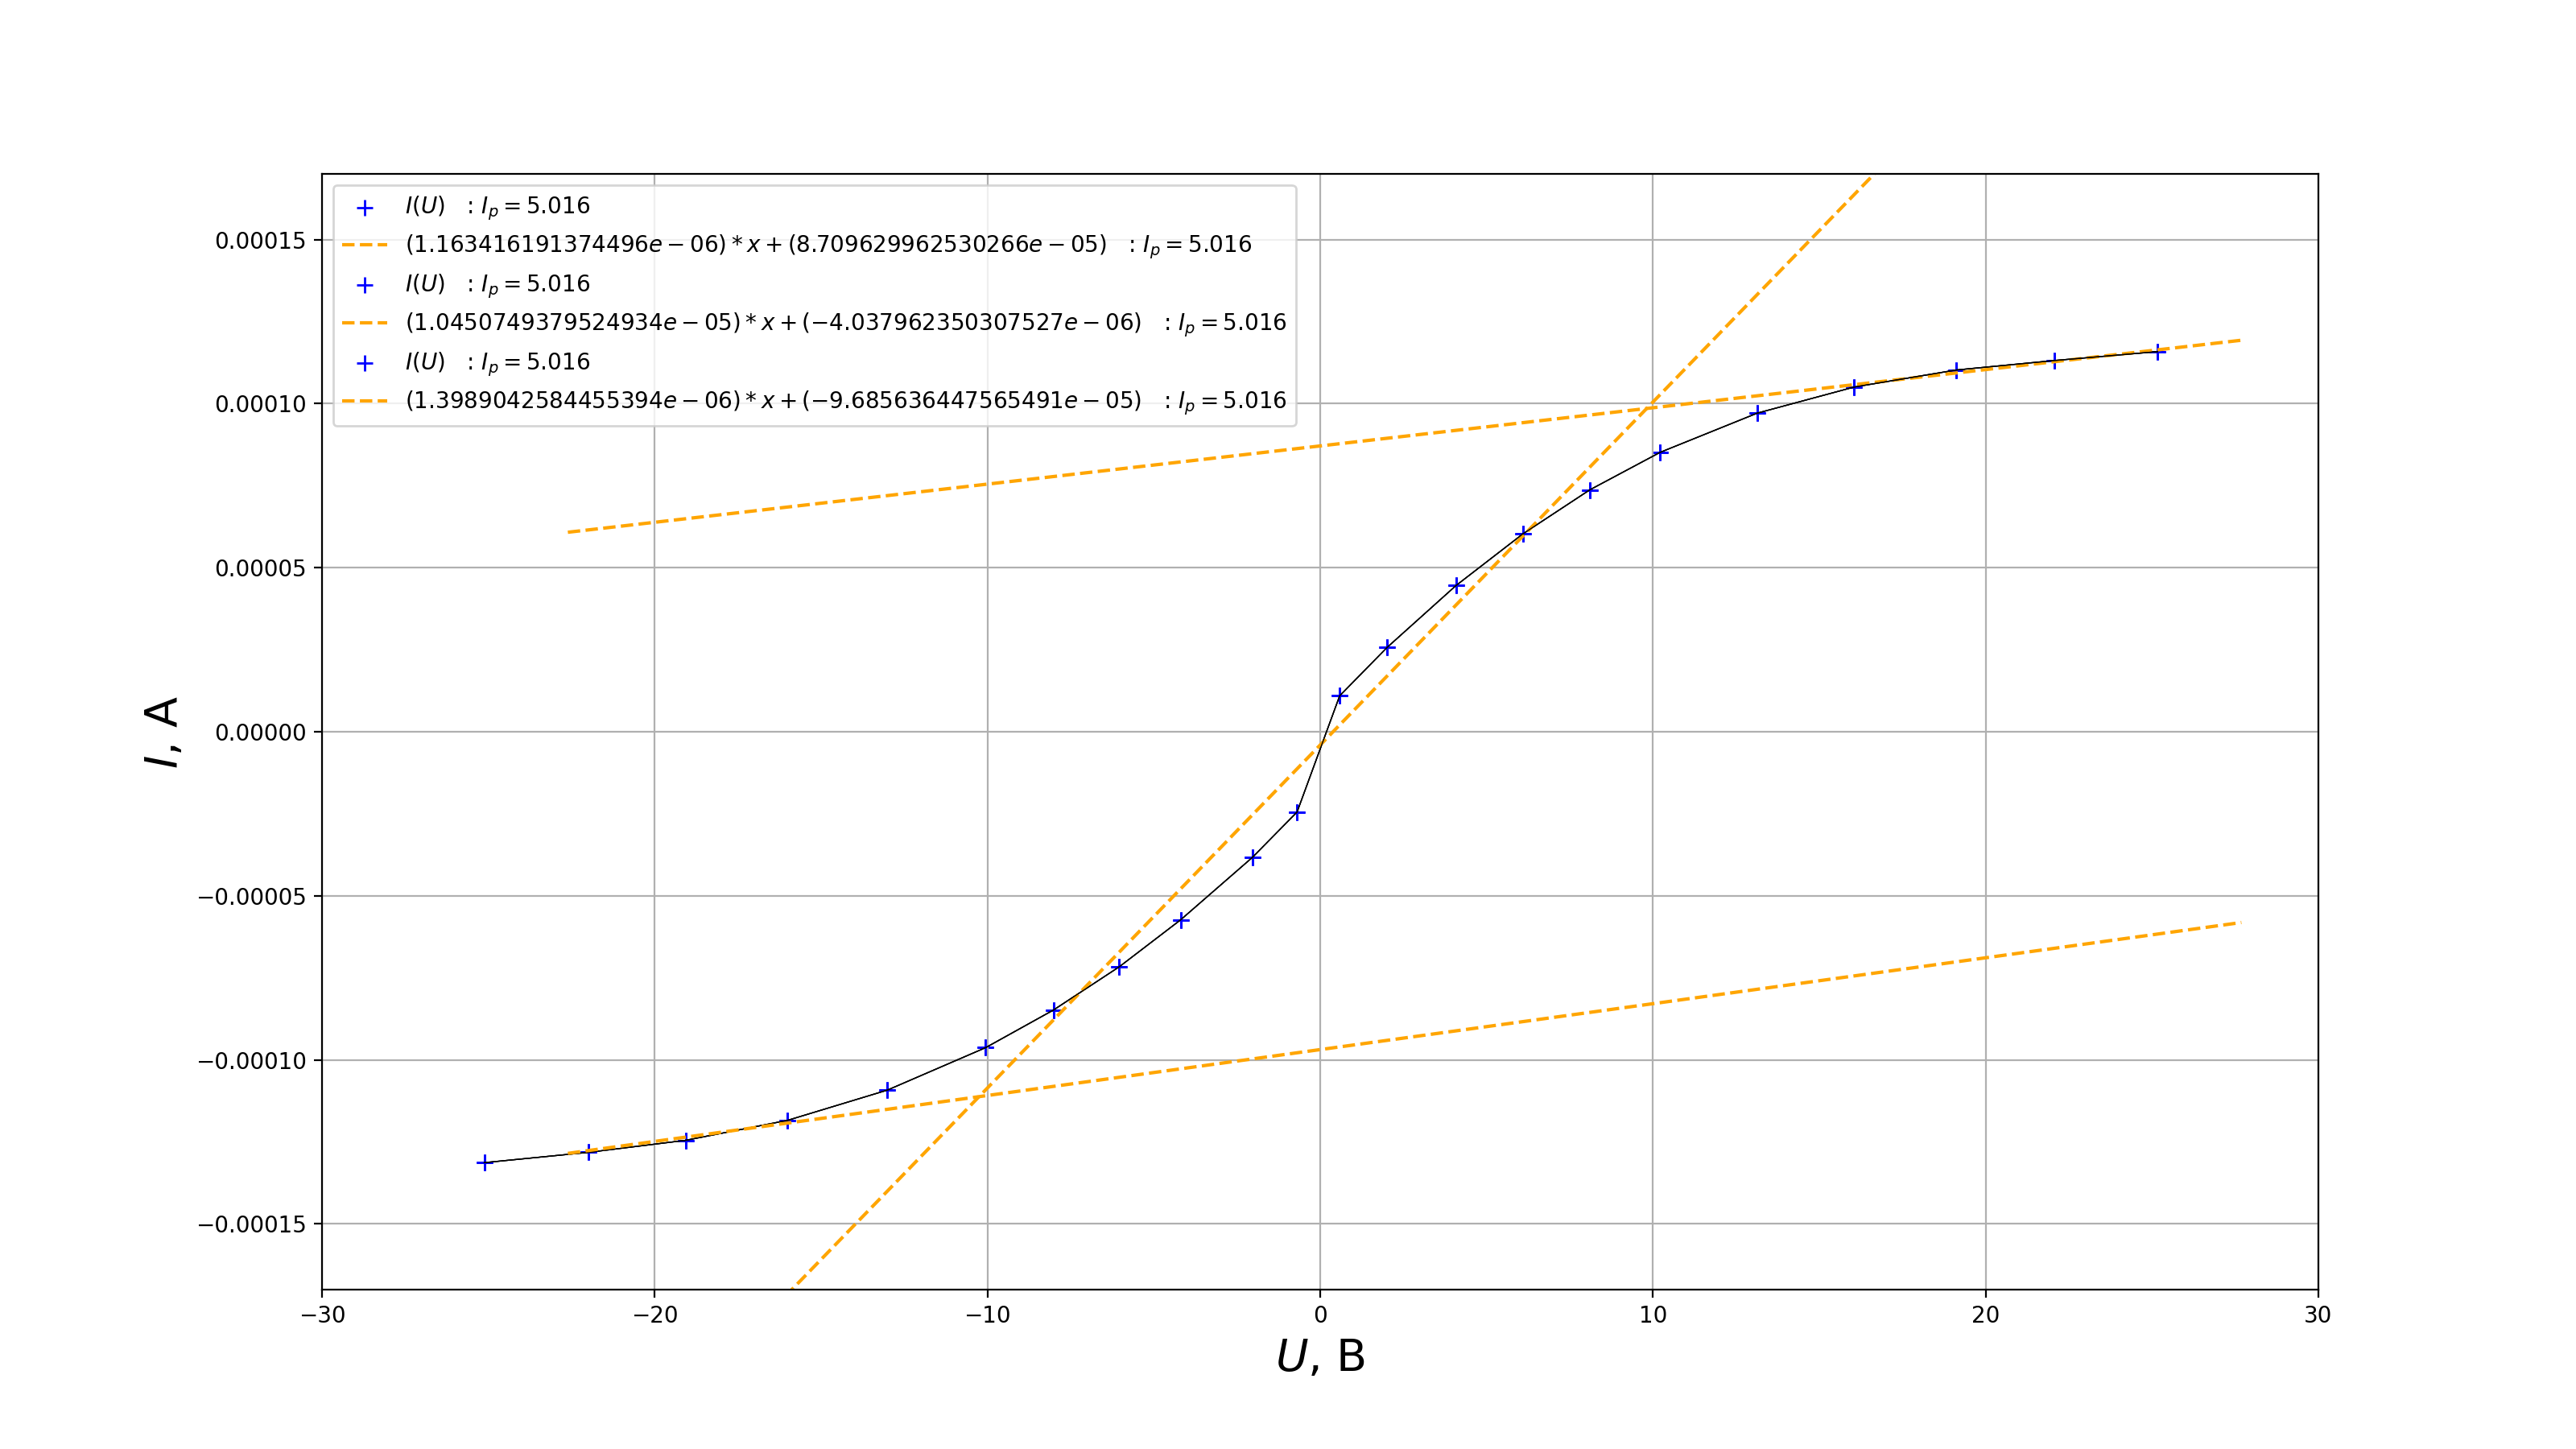
\includegraphics[width = \textwidth]{graph3.png}
    \caption{ВАХ зонда при $I_p = 5,02$ мА}
\end{figure}

\begin{figure}[H]
    \centering
    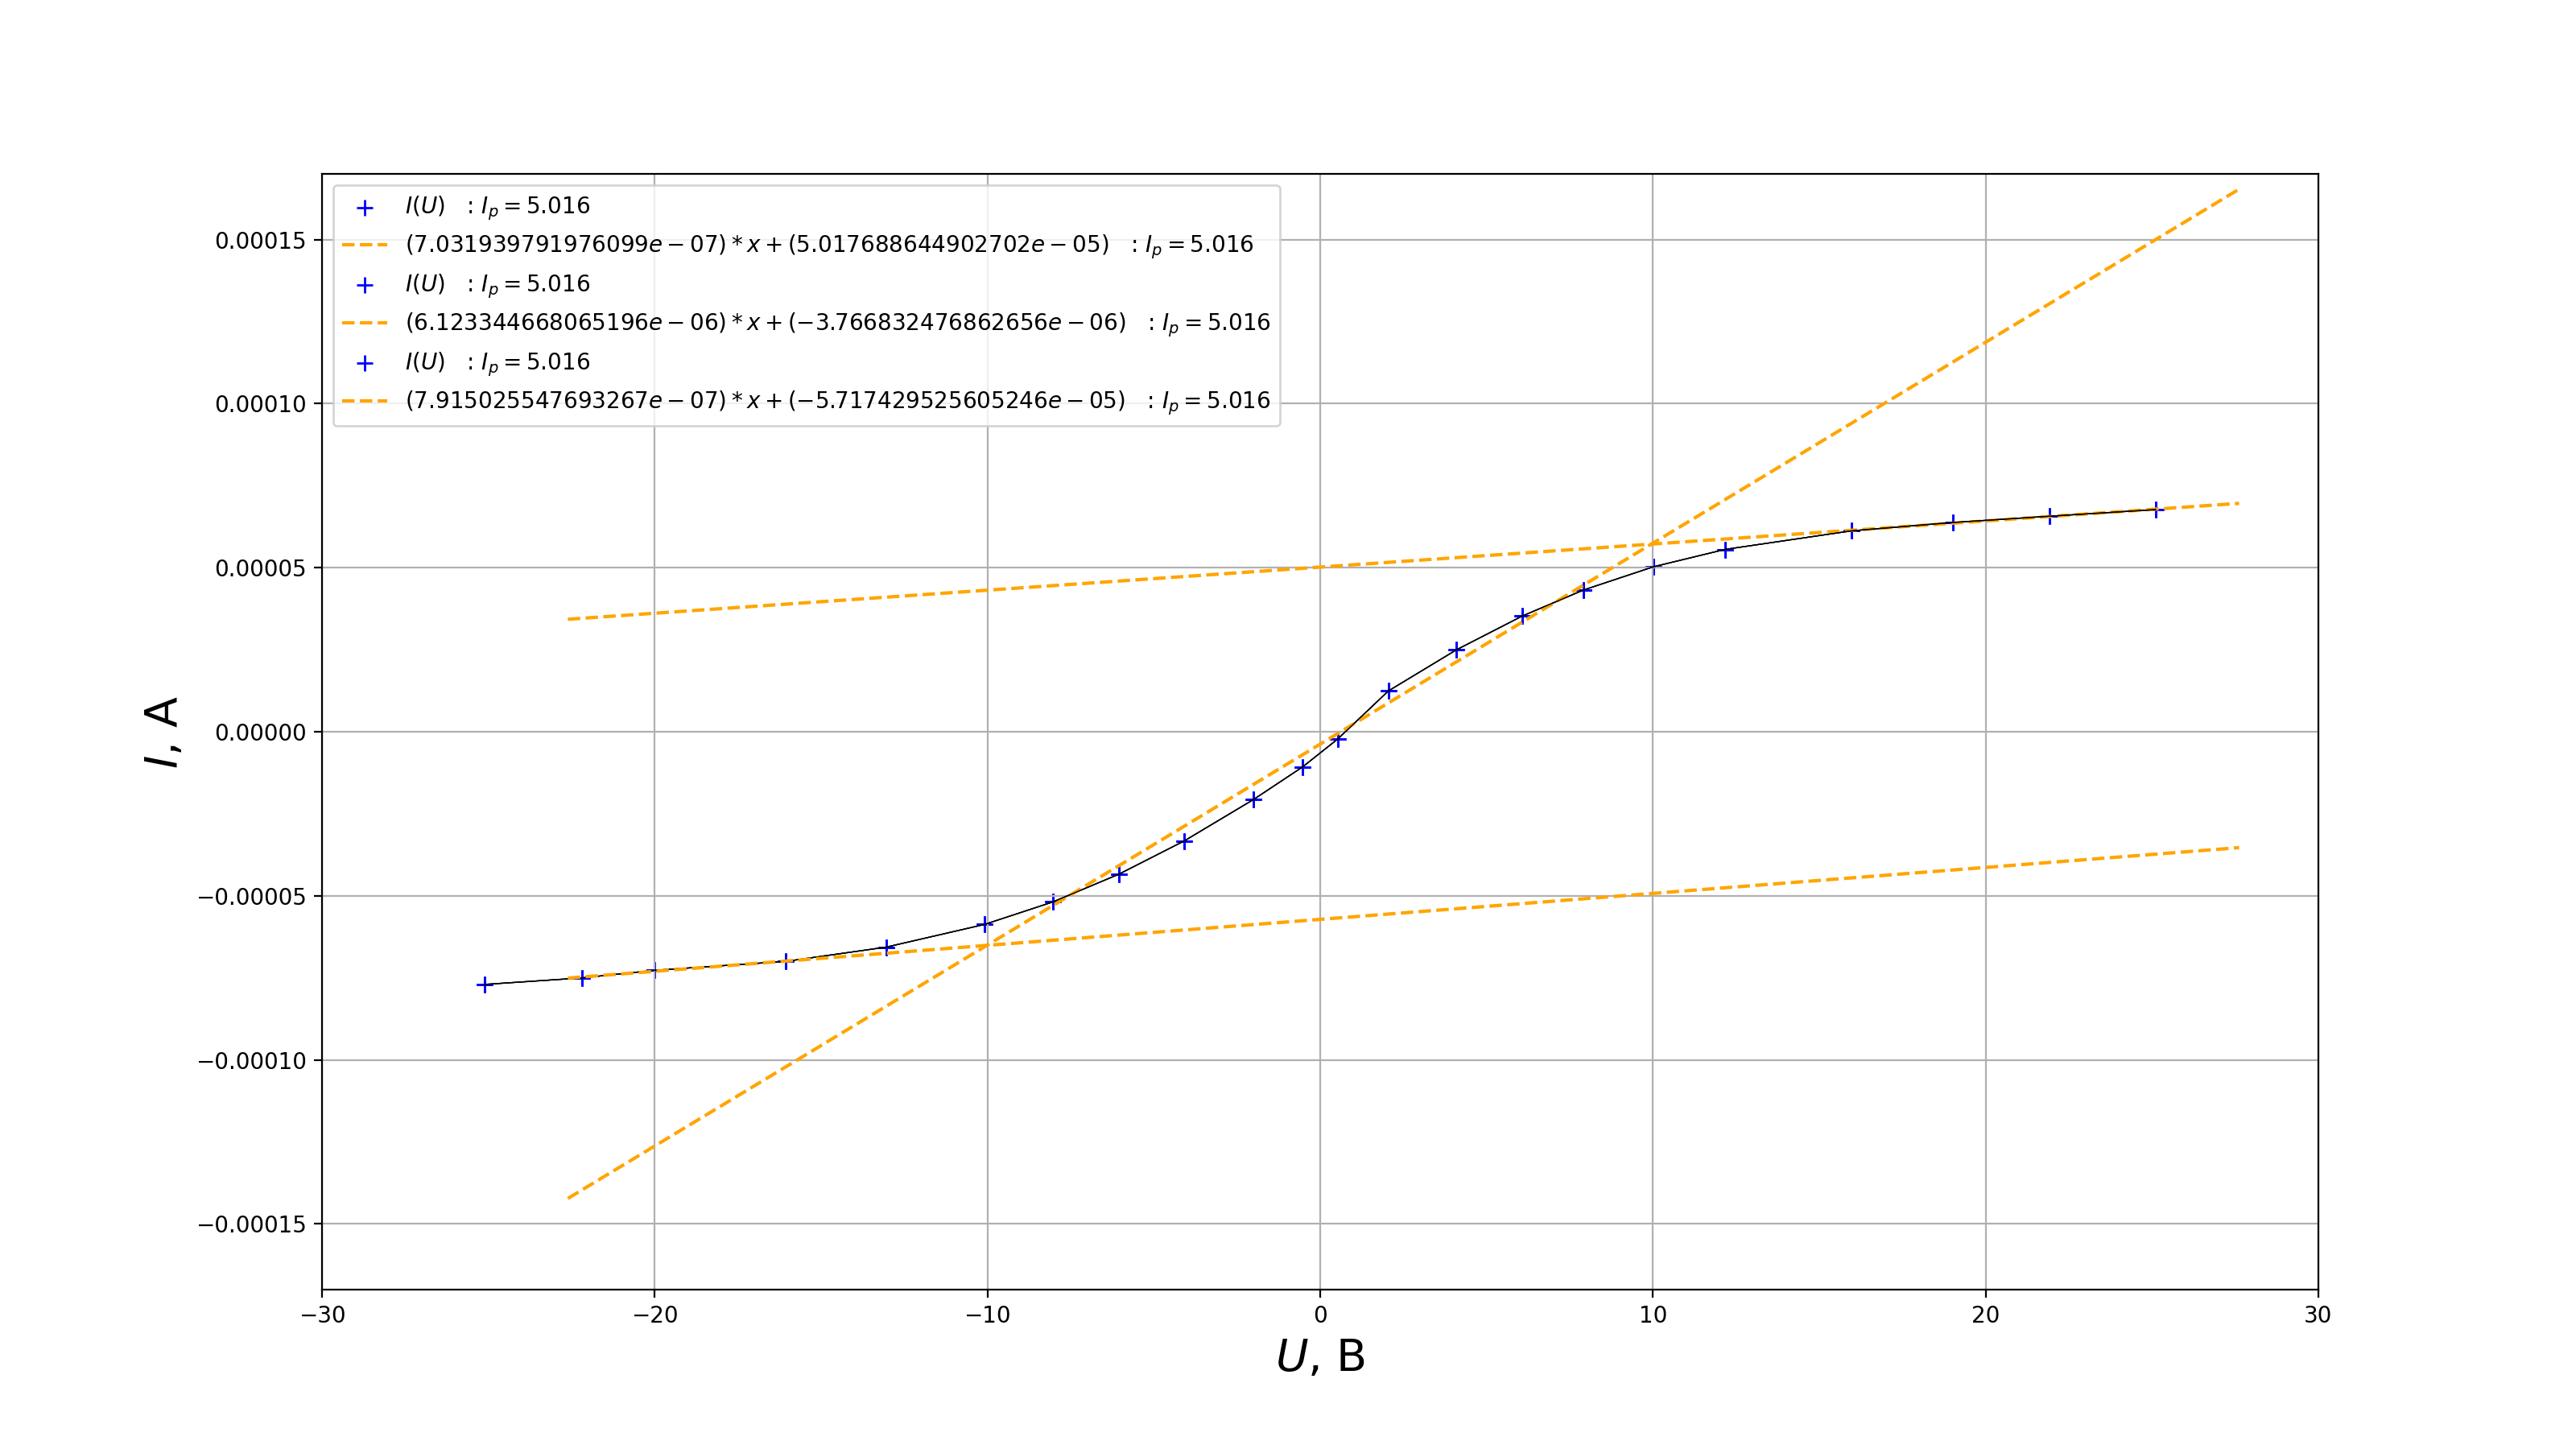
\includegraphics[width = \textwidth]{graph4.png}
    \caption{ВАХ зонда при $I_p = 3,06$ мА}
\end{figure}

\begin{figure}[H]
    \centering
    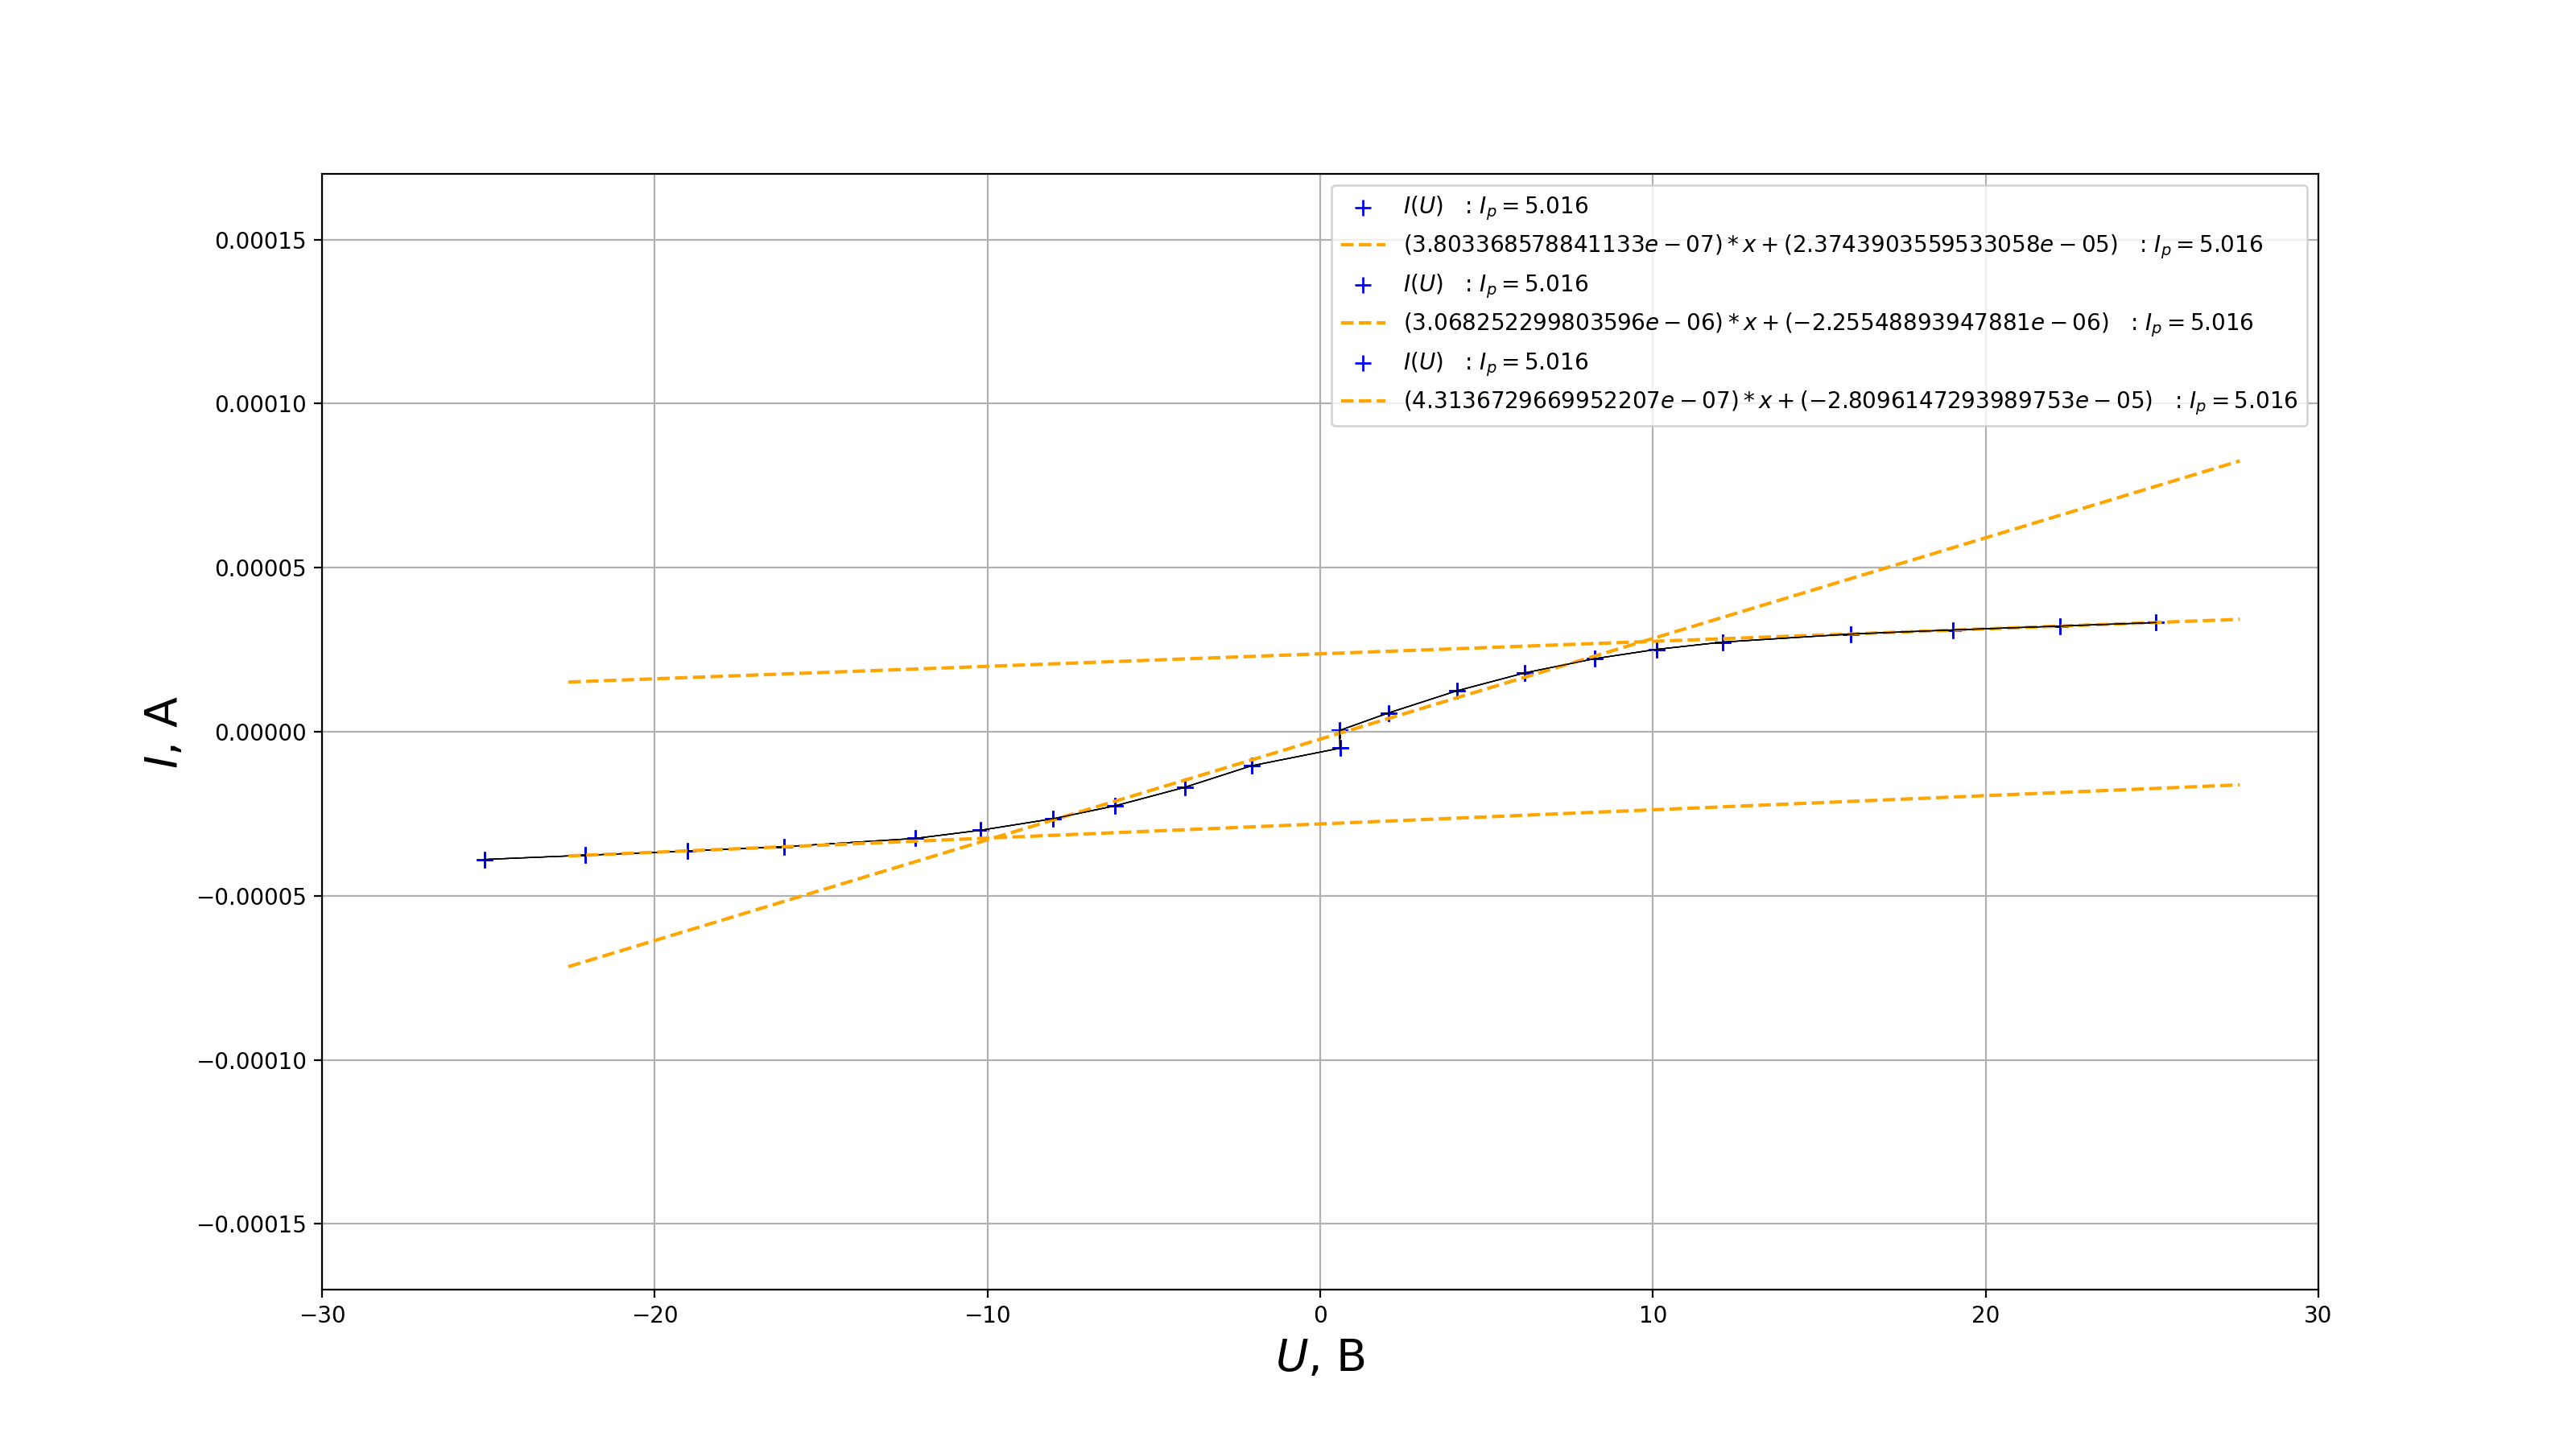
\includegraphics[width = \textwidth]{graph5.png}
    \caption{ВАХ зонда при $I_p = 1,47$ мА}
\end{figure}
\begin{table}[H]
    \centering
    \begin{tabular}{|c|c|c|c|c|c|c|}
        \hline
        $I_p$, мА  & $T_e$, $10^3$ К & $kT_e$, эВ & $n_e$, $10^{16}$ м$^{-3}$ & $\omega_p$, $10^9 \frac{\text{рад}}{c}$ & $r_{De}$, $10^{-3}$ cм & $r_D, 10^{-4}$ см  \\ \hline
        5.02   & $65.5\pm 4.5$ & $5.6 \pm 0.4$ & $5.17 \pm 0.37$                     & $12.8\pm 0.5$                   & $7.76\pm 0.28$    &   $5.25 \pm 0.19$            \\ \hline
        3.06   & $66.0\pm 3.3$ & $5.7 \pm 0.3$ & $3.95\pm 0.21$                     & $11.2\pm 0.3$                    & $8.92\pm 0.24$    &  $6.01 \pm 0.16$               \\ \hline
        1.47   & $50.6\pm 1.2$ & $4.4 \pm 0.1$ & $2.08\pm 0.03$                    & $8.1\pm 0.1$                     & $10.75 \pm 0.07$  &  $8.28 \pm 0.06$                 \\ \hline
    \end{tabular}
    \caption{Результаты вычислений}
\end{table}

$r_D$ рассчитываем в предположении, что $T_i \ll T_e, \ T_i \approx 300 K$.

Степень ионизации $\alpha$ рассчитаем из условия, что $P \approx 2$ торр. $\alpha = \dfrac{n_i}{n}$, где $P = nkT_i$
\begin{table}[H]
    \centering
    \begin{tabular}{|c|c|c|}
        \hline
        $I_p$, мА & $N_D$ & $\alpha, 10^{-7}$ \\ \hline
        5.02 & $31.4 \pm 4.1 $ & $8.03 \pm 0.58$ \\ \hline
        3.02 & $35.9 \pm 3.4$ & $6.13 \pm 0.33$ \\ \hline
        1.52 & $49.4 \pm 1.2$ & $3.23 \pm 0.04$ \\ \hline
    \end{tabular}
    \caption{Результаты вычислений}
\end{table}

\section*{Вывод}
В данной лабораторной работе мы исследовали состояние плазмы в тлеющем газовом разряде c помощью двойного зонда. Полученные результаты сходятся с указанными в лабораторной работе по порядку. Плазму в тлеющем разряде можно с хорошей точностью назвать идеальной, так как $N_D > 30 \gg 1$.
\end{document}
